\subsection{Funktionsweise der optischen Wellenleiter}
\label{subsec:poffunktionsweise}

Informationen werden mittels Intensitätsmodulation der Lichtstrahlen übertragen.
Dabei wird das Licht durch einen transparenten Kern gesendet, welcher von einem
Mantel umgeben ist (siehe \autoref{fig:pofprinzip}). Die Brechzahl $n$ des
Kerns ist dabei größer als die des Mantels, was zu einer
Totalreflexion\footnote{beinahe vollständige Reflexion von Licht an der
Grenzfläche zweier Materialien} des Lichts am Übergang vom Kern zum Mantel
führt. Die Laufzeitunterschiede zwischen dem schnellsten und dem langsamsten
Strahl beschränken die Bandbreite (siehe \autoref{fig:poflichtausbreitung}). Bei
kürzeren Strecken erhöhen sich die Bitraten, da sich die Unterschiede zwischen
den Laufzeiten verringern. Durch die Totalreflexion kann das Licht auch durch
Biegungen geleitet werden. \cite{pofacprinzip}

\ifthenelse{\boolean{showPics}}{
    \begin{figure}[h]
        \begin{center}
            \begin{minipage}[t]{0.45\textwidth}
                \begin{center}
                    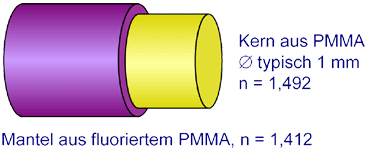
\includegraphics[width=0.9\textwidth]{Bilder/Optische_Wellenleiter_Die_Polymer_Optische_Faser/Funktionsweise/pofprinzip.png}
                    \caption[Aufbau einer polymer optischen Faser \newline \url{http://www.pofac.fh-nuernberg.de/pofac/de/was_sind_pof/images/pof_prinzip.png} (zuletzt aufgerufen am 19.09.2015)]{Aufbau einer polymer \\optischen Faser}
                    \label{fig:pofprinzip}
                \end{center}
            \end{minipage}
            \hspace{0.025\textwidth}
            \begin{minipage}[t]{0.45\textwidth}
                \begin{center}
                    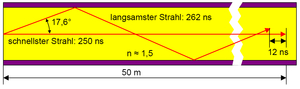
\includegraphics[width=0.9\textwidth]{Bilder/Optische_Wellenleiter_Die_Polymer_Optische_Faser/Funktionsweise/poflichtausbreitung.png}
                    \caption[Ausbreitung von Licht in einer polymer optischen Faser \newline \url{http://www.pofac.info/typo3temp/pics/7eee584dce.jpg} (zuletzt aufgerufen am 19.09.2015)]{Ausbreitung von Licht in einer polymer optischen Faser}
                    \label{fig:poflichtausbreitung}
                \end{center}
            \end{minipage}
        \end{center}
    \end{figure}
}{}
